\documentclass[a4paper, 11pt]{article}
\usepackage[polish]{babel}
\usepackage[T1]{fontenc}
\usepackage{hyperref}
\usepackage{array}
\usepackage{amssymb}
\hypersetup{
    colorlinks,
    citecolor=black,
    filecolor=black,
    linkcolor=black,
    urlcolor=black
}
\usepackage{graphicx}

\usepackage{tikz}
\usetikzlibrary{fit,arrows,matrix,positioning, calc, shapes.gates.logic.IEC, shapes.gates.logic.US}
\tikzstyle{branch}=[fill,shape=circle,minimum size=3pt,inner sep=0pt]


\title{%
       \large Sprawozdanie Laboratorium PTC \\
       \huge Proste Układy Kombinacyjne}

\author{Stanisław Fiedler 160250}
\date{LAB 1, 7 października 2024}

\begin{document}

\maketitle
\tableofcontents

\section{Zadanie 3}
Koder priorytetowy jest nieco podobny do układu z zadania 2.
Układ ma 3 wejścia X0, X1, X2 i 3 wyjścia Y0, Y1, GS (Got Something).
Jezeli jedno lub więcej wejść jest aktywne (stan „1”), to GS=”1” a na wyjściach Y1, Y0 pojawia się zakodowany (naturalny kod binarny) numer aktywnego wejścia znajwyższą wagą. Kodowanie: 00, 01, 10.
Wagi wejść i wyjść: X2 najwyższa X0 najniższa. Y1 najwyższa,
Y0 najniższa.

\begin{enumerate}
	\item Sporządź tablice wartości funkcji Y1, Y0 i GS;
	\item Korzystając z siatki Karnaugha zminimalizuj funkcje Y1, Y0, GS;
	\item Narysuj schemat układu wykorzystując bramki AND, OR, NOT;
	\item Zasymuluj działanie układu wykorzystując Logisim;
	\item Przekształć układ, tak aby można go było zrealizować korzystając wyłącznie z 2-wejściowych
	      bramek NAND;
	\item Zasymuluj działanie układu z punktu 5 wykorzystując Logisim.
\end{enumerate}

\subsection{Tablica wartości funkcji Y1, Y0 i GS}\label{sub:tablicawartosci} % (fold)

\begin{center}
	\[
		\begin{array}{ | c | c | c || c | c | c | }
			\hline
			X_2 & X_1 & X_0 & Y_1 & Y_0 & GS \\
			\hline\hline
			0   & 0   & 0   & 0   & 0   & 0  \\
			0   & 0   & 1   & 0   & 0   & 1  \\
			0   & 1   & 0   & 0   & 1   & 1  \\
			0   & 1   & 1   & 0   & 1   & 1  \\
			1   & 0   & 0   & 1   & 0   & 1  \\
			1   & 0   & 1   & 1   & 0   & 1  \\
			1   & 1   & 0   & 1   & 0   & 1  \\
			1   & 1   & 1   & 1   & 0   & 1  \\
			\hline
		\end{array}
	\]
\end{center}

% subsection  (end)

\subsection{Siatka Karnaugha}\label{sub:siatka_} % (fold)
\begin{center}
	\[ Y_1 \]
	\begin{tikzpicture}
		\matrix (Y1) [matrix of math nodes, nodes in empty cells, nodes={minimum height=1cm, minimum width=1cm, anchor=center}, column 1/.style={nodes={minimum height=1cm, minimum width=2cm, anchor=center}}] (m)
		{
				{} & 00 & 01 & 11 & 10 \\
				0             & 0  & 0  & 0  & 0  \\
				1             & 1  & 1  & 1  & 1  \\
			};
		\draw[double distance=2pt] (m-1-2.north west) -- (m-3-2.south west);
		\draw[double distance=2pt] (m-1-1.south west) -- (m-1-5.south east);
		\node[fit={(m-3-2.north west) (m-3-5.south east)},
			thick, inner sep=0pt, rounded corners=1mm,
			draw=blue ]{};
		\draw (m-1-1.north west) -- (m-1-1.south east);
		\node[anchor=south west, font=\small] at ($(m-1-1.center) + (-0.2,-0.1)$) {$X_1X_0$};
		\node[anchor=north east, font=\small] at ($(m-1-1.center) + (-0.2,0.2)$) {$X_2$};
	\end{tikzpicture}
	\raisebox{1cm}{\Large $ \quad Y_1 = X_2 $}
\end{center}

\begin{center}
	\[ Y_0 \]
	\begin{tikzpicture}
		\matrix (Y1) [matrix of math nodes, nodes in empty cells, nodes={minimum height=1cm, minimum width=1cm, anchor=center}, column 1/.style={nodes={minimum height=1cm, minimum width=2cm, anchor=center}}] (m)
		{
				{} & 00 & 01 & 11 & 10 \\
				0         & 0  & 0  & 1  & 1  \\
				1         & 0  & 0  & 0  & 0  \\
			};
		\draw[double distance=2pt] (m-1-2.north west) -- (m-3-2.south west);
		\draw[double distance=2pt] (m-1-1.south west) -- (m-1-5.south east);;
		\node[fit={(m-2-4.north west) (m-2-5.south east)},
			thick, inner sep=0pt, rounded corners=1mm,
			draw=blue ]{};
		\draw (m-1-1.north west) -- (m-1-1.south east);
		\node[anchor=south west, font=\small] at ($(m-1-1.center) + (-0.2,-0.1)$) {$X_1X_0$};
		\node[anchor=north east, font=\small] at ($(m-1-1.center) + (-0.2,0.2)$) {$X_2$};
	\end{tikzpicture}
	\raisebox{1cm}{\Large $ \quad Y_0 = \bar{X_2}X_1 $}
\end{center}

\begin{center}
	\[ GS \]
	\begin{tikzpicture}
		\matrix (Y1) [matrix of math nodes, nodes in empty cells, nodes={minimum height=1cm, minimum width=1cm, anchor=center}, column 1/.style={nodes={minimum height=1cm, minimum width=2cm, anchor=center}}] (m)
		{
				{} & 00 & 01 & 11 & 10 \\
				0             & 0  & 1  & 1  & 1  \\
				1             & 1  & 1  & 1  & 1  \\
			};
		\draw[double distance=2pt] (m-1-2.north west) -- (m-3-2.south west);
		\draw[double distance=2pt] (m-1-1.south west) -- (m-1-5.south east);;
		\node[fit={(m-2-4.north west) (m-3-5.south east)},
			thick, inner sep=0pt, rounded corners=1mm,
			draw=green ]{};
		\node[fit={(m-2-3.north west) (m-3-4.south east)},
			thick, inner sep=0pt, rounded corners=1mm,
			draw=blue ]{};
		\node[fit={(m-3-2.north west) (m-3-5.south east)},
			thick, inner sep=0pt, rounded corners=1mm,
			draw=red ]{};
		\draw (m-1-1.north west) -- (m-1-1.south east);
		\node[anchor=south west, font=\small] at ($(m-1-1.center) + (-0.2,-0.1)$) {$X_1X_0$};
		\node[anchor=north east, font=\small] at ($(m-1-1.center) + (-0.2,0.2)$) {$X_2$};
	\end{tikzpicture}
	\raisebox{1cm}{\Large $ \quad GS = X_2 + X_1 + X_0 $}
\end{center}
% subsection Siatka  (endLahaina)

\subsection{Schemat AND, OR, NOT}\label{sub:schemat_and_or_not} % (fold)
\begin{tikzpicture}[label distance=2mm, scale=1.4, transform shape]
	\node (x2) at (1,0) {$X_2$};
	\node (x1) at (2,0) {$X_1$};
	\node (x0) at (3,0) {$X_0$};

	\node[not gate US, draw, rotate=-90] at ($(x2)+(0.5,-1)$) (not2) {};

	\node (y1) at ($(x0)+(4,-2)$) {$Y_1$};
	\node (y0) at ($(x0)+(4,-3)$) {$Y_0$};
	\node (GS) at ($(x0)+(4,-4)$) {$GS$};

	\node[and gate US, draw, logic gate inputs=nn] at ($(x0)+(2,-3)$) (and1) {};
	\node[or gate US, draw, logic gate inputs=nnn] at ($(x0)+(2,-4)$) (or1) {};

	\foreach \i in {2}
		{
			\path (x\i) -- coordinate (punt\i) (x\i |- not\i.input);
			\draw (punt\i) node[branch] {} -| (not\i.input);
		}

	\draw (and1.output) -- (y0);
	\draw (or1.output) -- (GS);
	\draw (x2) |- (or1.input 3);
	\draw (x2 |- y1) node[branch] {} -- (y1);
	\draw (x1) |- (or1.input 2);
	\draw (x0) |- (or1.input 1);
	\draw (not2) |- (and1.input 2);
	\draw (x1 |- and1.input 1) node[branch] {} -- (and1.input 1);


\end{tikzpicture}
% subsection Schemat AND, OR, NOT (end)

\subsection{Symulacja Logisim AND, OR, NOT}\label{sub:symulacja_logisim} % (fold)
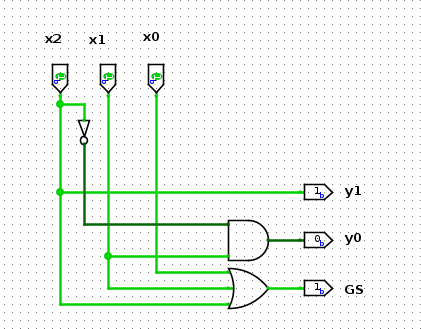
\includegraphics[scale = 0.75]{images/and_or_not.png}
% subsection Symulacja Logisim (end)

\subsection{Schemat NAND}\label{sub:schemat_nand} % (fold)
\begin{tikzpicture}[label distance=2mm, scale=1.4, transform shape]
	\node (x2) at (1,0) {$X_2$};
	\node (x1) at (2.5,0) {$X_1$};
	\node (x0) at (4,0) {$X_0$};

	\node[nand gate US, draw, rotate=-90, logic gate inputs=nn] at ($(x2)+(0.5,-1)$) (nand2) {};
	\node[nand gate US, draw, rotate=-90, logic gate inputs=nn] at ($(x1)+(0.5,-1)$) (nand1) {};
	\node[nand gate US, draw, rotate=-90, logic gate inputs=nn] at ($(x0)+(0,-1)$) (nand0) {};

	\node (y1) at ($(x0)+(6,-2)$) {$Y_1$};
	\node (y0) at ($(x0)+(6,-3)$) {$Y_0$};
	\node (GS) at ($(x0)+(6,-4.5)$) {$GS$};

	\node[nand gate US, draw, logic gate inputs=nn] at ($(x0)+(1,-3)$) (nand3) {};
	\node[nand gate US, draw, logic gate inputs=nn] at ($(x0)+(2.5,-3)$) (nand4) {};

	\node[nand gate US, draw, logic gate inputs=nn] at ($(x0)+(1,-4)$) (nand5) {};
	\node[nand gate US, draw, logic gate inputs=nn] at ($(x0)+(2.5,-4)$) (nand6) {};
	\node[nand gate US, draw, logic gate inputs=nn] at ($(x0)+(4,-4.5)$) (nand7) {};

	\draw (x2) |- (y1);
	\draw (nand2.output) |- (nand7.input 2);
	\draw (nand2.output |- nand3.input 2) node[branch] {} -- (nand3.input 2);
	\draw (x1) |- (nand3.input 1);
	\draw (nand1.output) |- (nand5.input 2);
	\draw (nand0.output) |- (nand5.input 1);
	\draw (nand4.output) -- (y0);
	\draw (nand7.output) -- (GS);
	\draw (nand6.output) -- ++(0.3,0) |- (nand7.input 1);
	\draw (nand3.output) -| ++(0.3,0) node[branch] {} |- (nand4.input 1);
	\draw (nand3.output) -| ++(0.3,0) |- (nand4.input 2);
	\draw (nand5.output) -| ++(0.3,0) node[branch] {} |- (nand6.input 1);
	\draw (nand5.output) -| ++(0.3,0) |- (nand6.input 2);
	\draw (x0) |- ++(0,-0.5) -| (nand0.input 1);
	\draw (x0) |- ++(0,-0.5) -| (nand0.input 2);
	\draw ($(x2)+(0,-0.5)$) node[branch] {} -| (nand2.input 1);
	\draw ($(x2)+(0,-0.5)$) -| node[branch] {} (nand2.input 2);
	\draw ($(x1)+(0,-0.5)$) node[branch] {} -| (nand1.input 1);
	\draw ($(x1)+(0,-0.5)$) -| node[branch] {} (nand1.input 2);

\end{tikzpicture}
% subsection Schemat NAND (end)

\subsection{Symulacja Logisim NAND}\label{sub:symulacja_logisim_nand} % (fold)

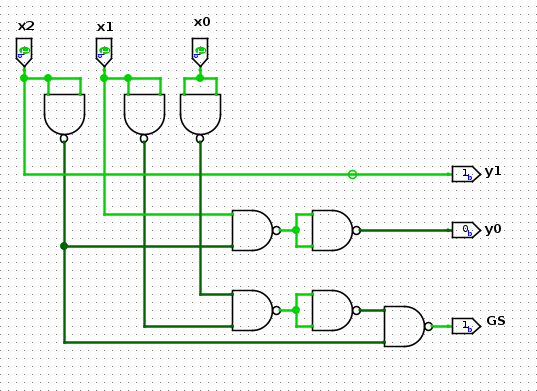
\includegraphics[scale = 0.75]{images/nand.png}
% subsection Symulacja Logisim NAND (end)

\end{document}
